\documentclass[aspectratio=169]{beamer}
\usepackage{color,amsmath}
\usepackage{subfigure}
\usepackage{booktabs}
\usepackage{framed}
\usepackage{comment}
\usepackage{hyperref}
\usepackage{ulem}

\usepackage{hyperref}
\hypersetup{
    colorlinks=true,
    linkcolor=blue,
    filecolor=magenta,      
    urlcolor=cyan,
}

%%%%%%%%%%%%%%%%%%%%%%%%%%
\title[]{\textcolor{gray}{[Introduction to mass collaboration], [Human computation], [Open call],} [Distributed data collection], \textcolor{gray}{\newline [Fragile Families Challenge]}}
\author[]{Matthew J. Salganik\\Department of Sociology\\Princeton University}
\date[]{%Summer Institutes in Computational Social Science\\2020
%\vfill
%\begin{flushleft}
%{\scriptsize
%The Summer Institutes in Computational Social Science is supported by grants from the Russell Sage Foundation and the Alfred P. Sloan Foundation.}
%\end{flushleft}
\begin{flushright}

\includegraphics[width=0.1\textwidth]{figures/cc-by.png}
\end{flushright}
}
\begin{document}
%%%%%%%%%%%%%%%%%%%%%%%%%%
\frame{\titlepage}
%%%%%%%%%%%%%%%%%%%%%%%%%%
\begin{frame}

\begin{columns}
\begin{column}{.40\textwidth}
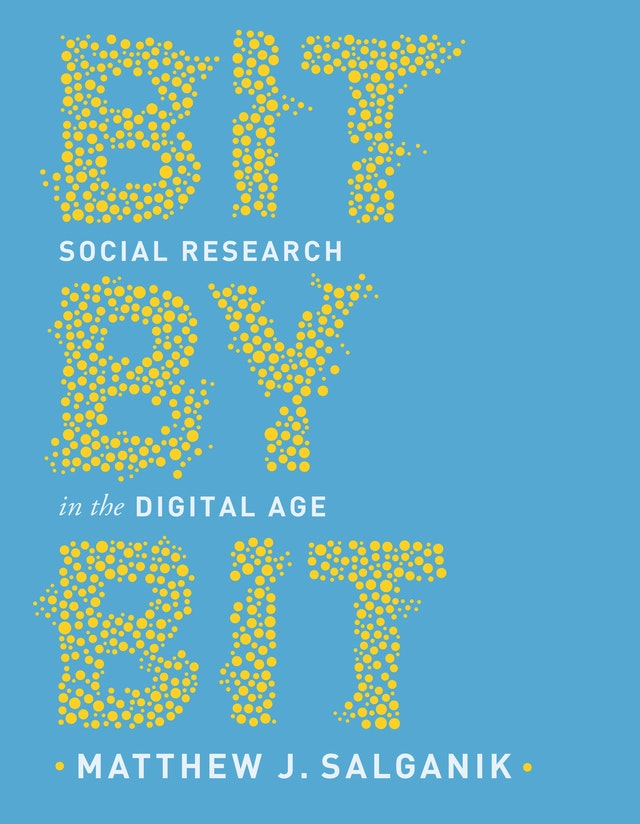
\includegraphics[width=\textwidth]{figures/salganik_bit_2018_cover}
\end{column}%

\hfill%

\begin{column}{.60\textwidth}
1) Introduction \\
2) Observing behavior \\
3) Asking questions \\
4) Running experiments \\
\textcolor{blue}{5) Mass collaboration} \\
6) Ethics \\
7) The future \\
\end{column}%
\end{columns}

\end{frame}
%%%%%%%%%%%%%%%%%%%%%%%%%
\begin{frame}

\begin{center}
\only<1>{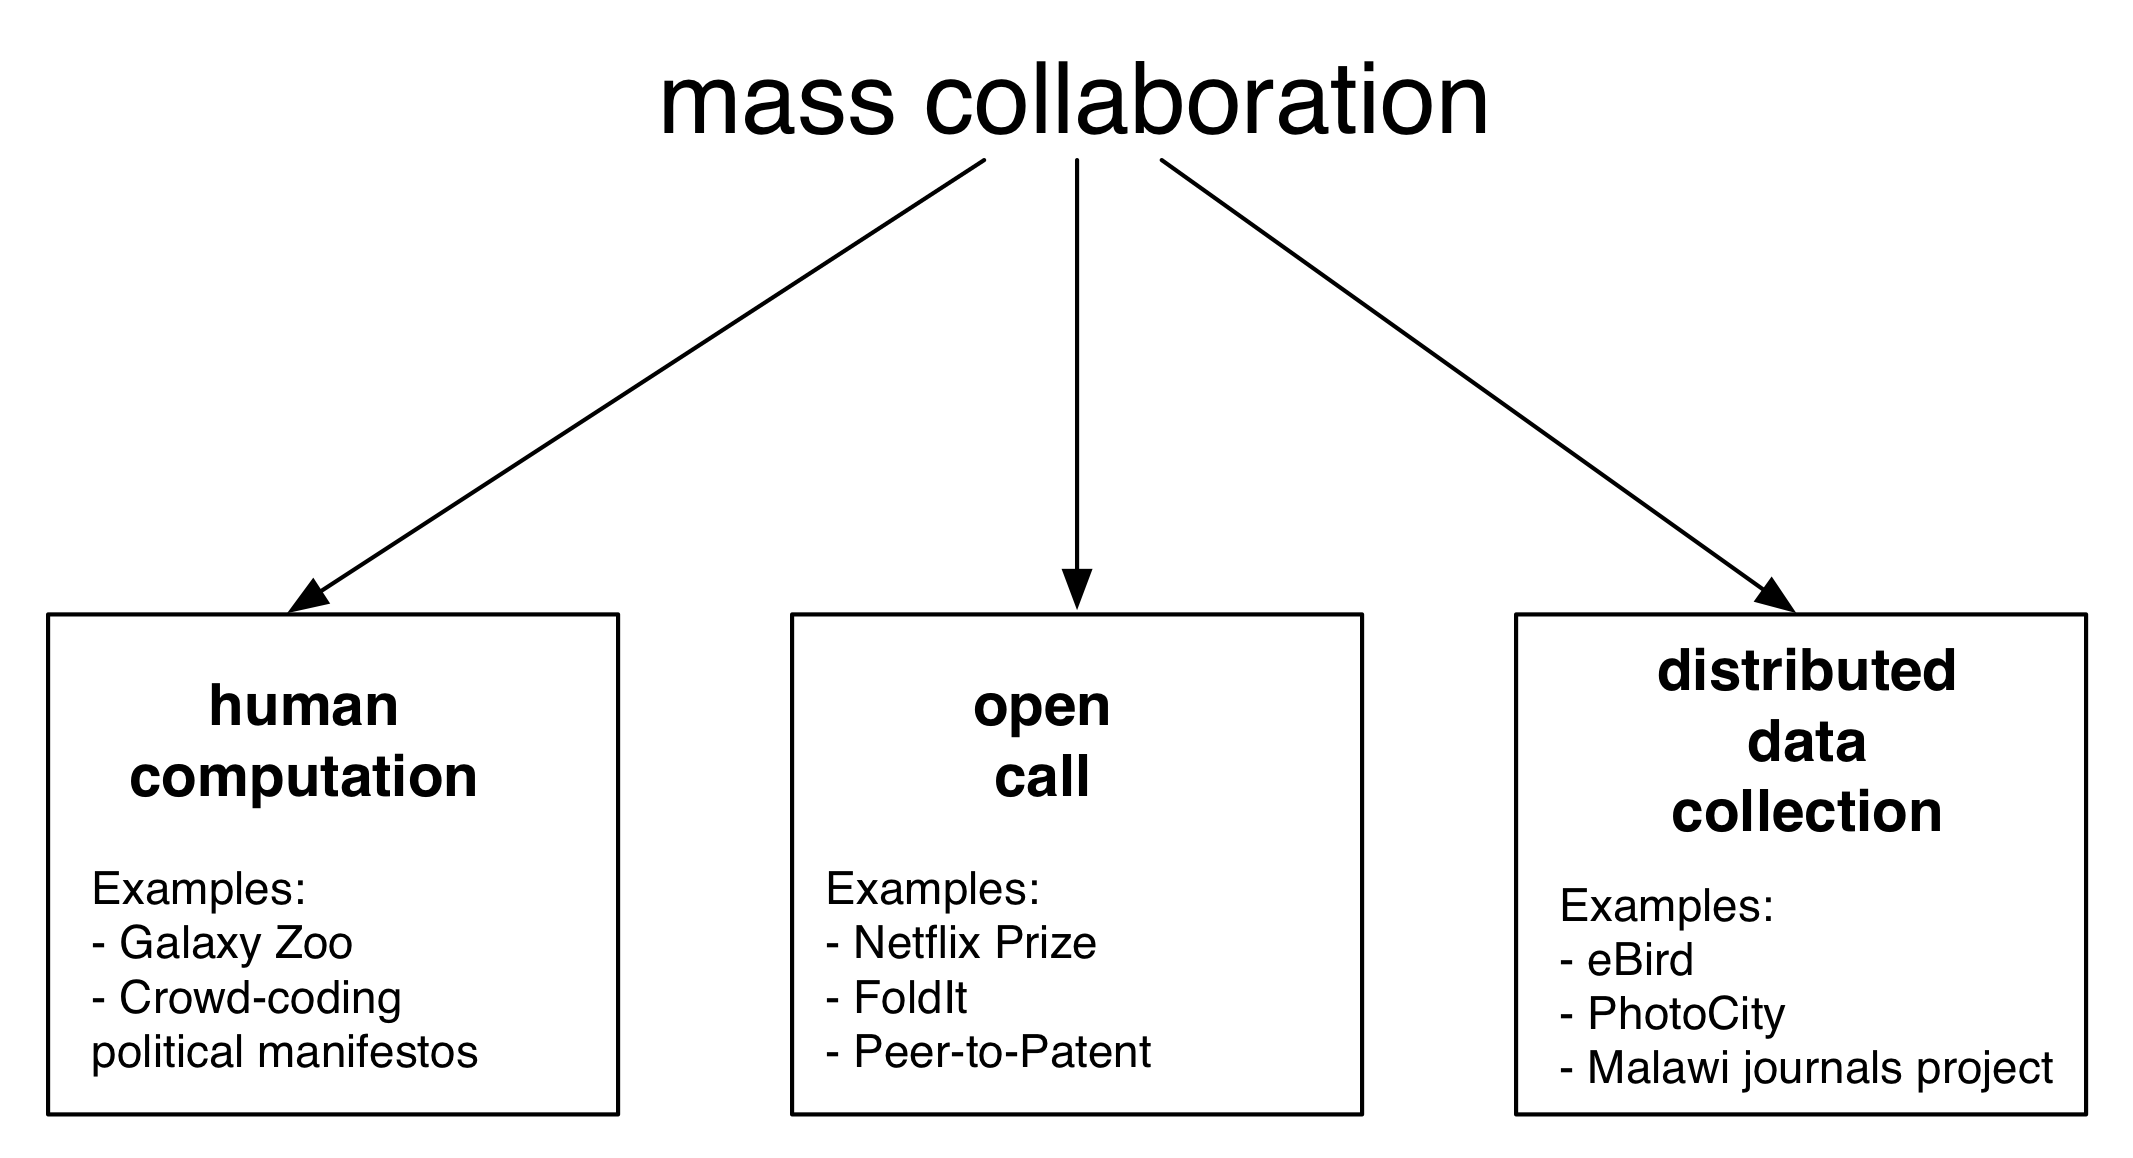
\includegraphics[width=0.9\textwidth]{figures/mass_collaboration_schematic}}
\only<2>{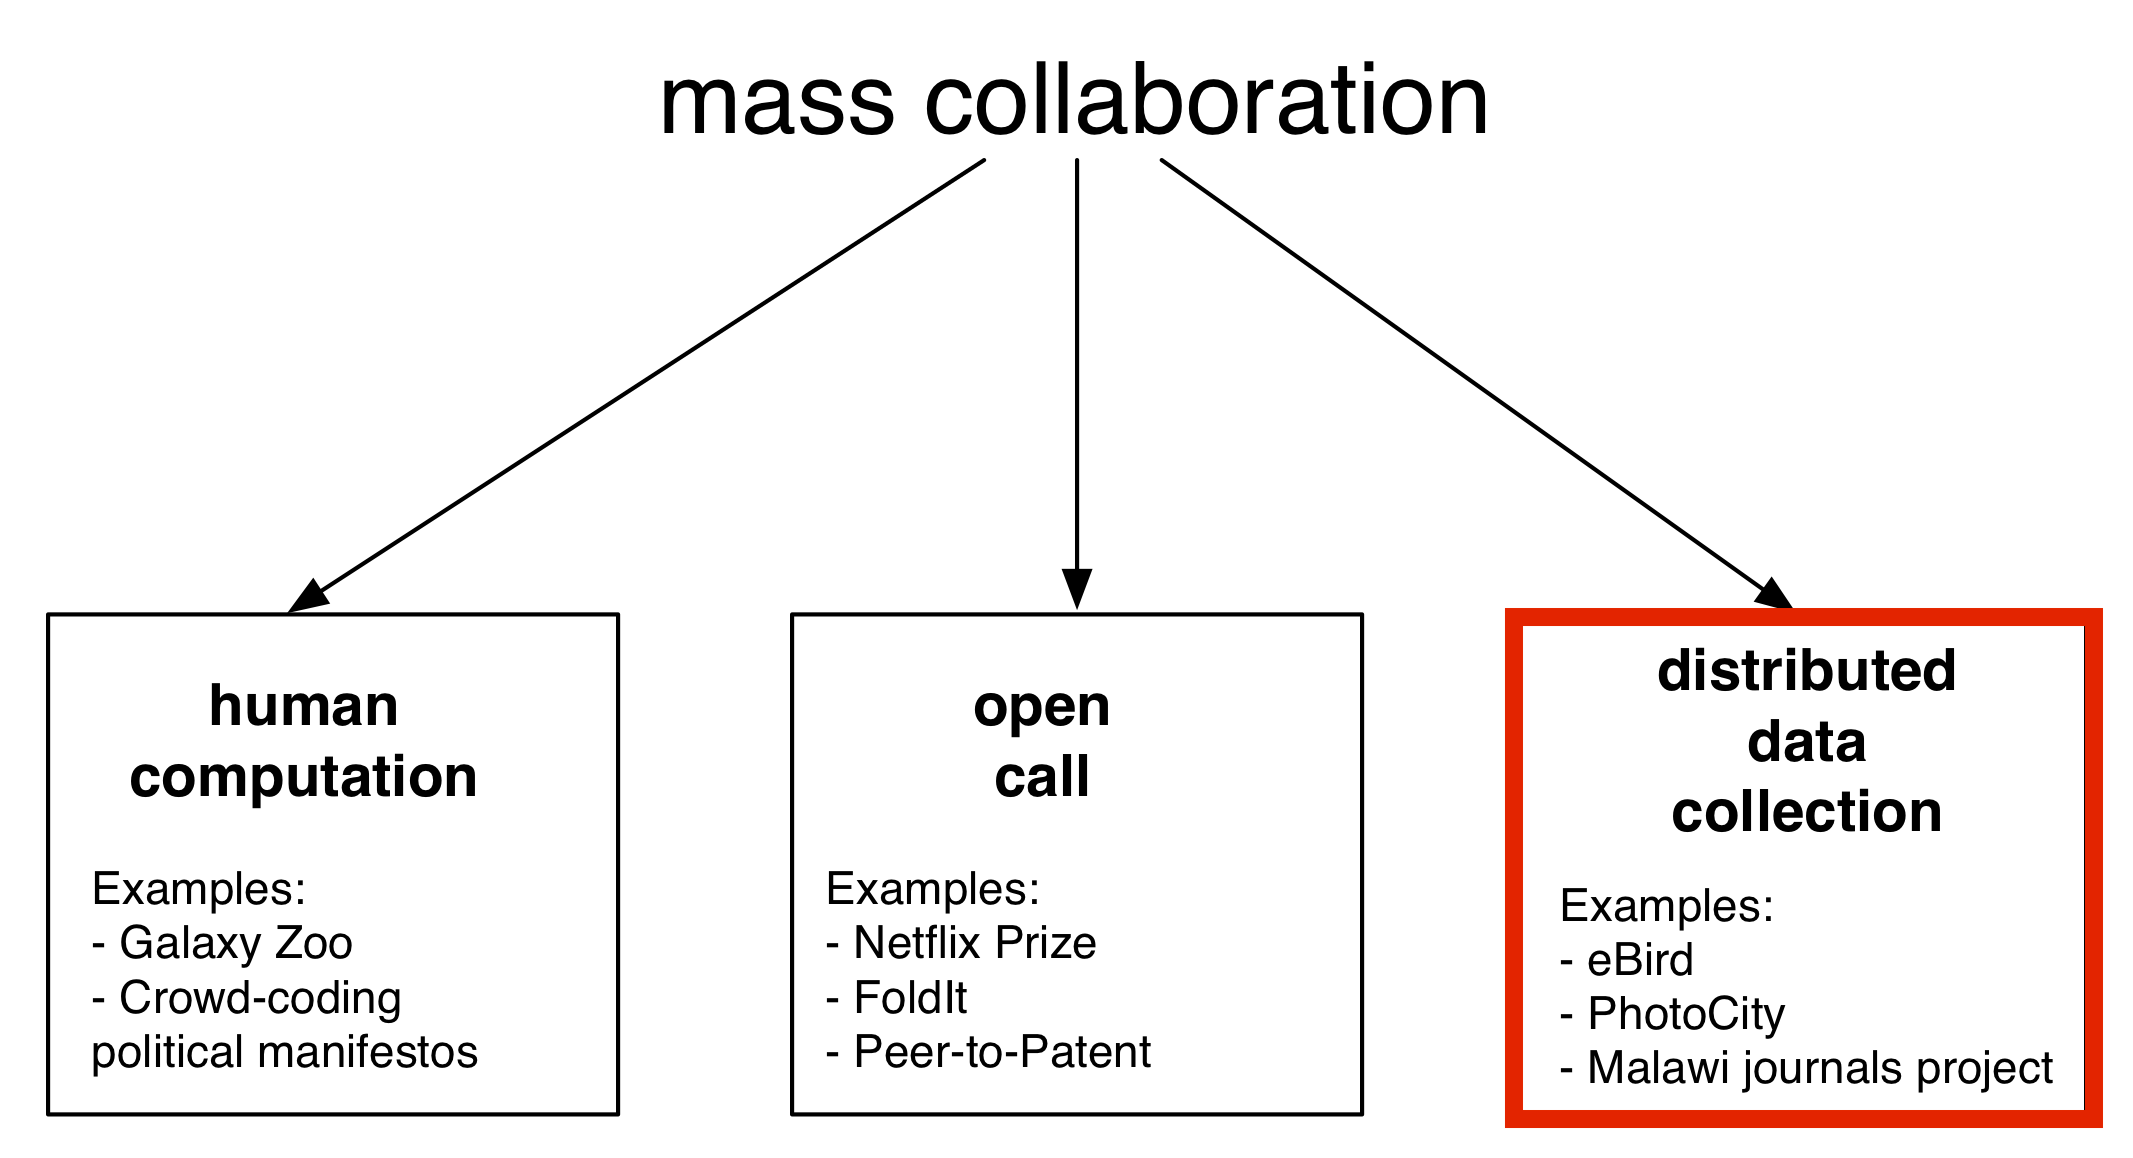
\includegraphics[width=0.9\textwidth]{figures/mass_collaboration_schematic_dist_data_collection}}
\end{center}

\vfill
Fig 5.4 (\href{https://www.bitbybitbook.com/}{Salganik 2018})
\end{frame}

%%%%%%%%%%%%%%%%%%%%%%%%%%
\begin{frame}

Distributed data collection:
\begin{itemize}
\item people can be where the researchers can't
\pause
\item scale that researcher cannot match
\pause
\item sometimes hard to separate from human computation
\end{itemize}

\end{frame}
%%%%%%%%%%%%%%%%%%%%%%%%%%
\begin{frame}

Claims:
\begin{itemize}
\item Distributed data collection is possible for real research
\pause
\item Sampling and data quality concerns are not insurmountable 
\pause
\item Distributed data collection can produce different---not just cheaper---data 
\end{itemize}

\end{frame}
%%%%%%%%%%%%%%%%%%%%%%%%%%
\begin{frame}

\begin{center}

\includegraphics[width=0.5\textwidth]{figures/ebird_logo}
\end{center}
\begin{center}
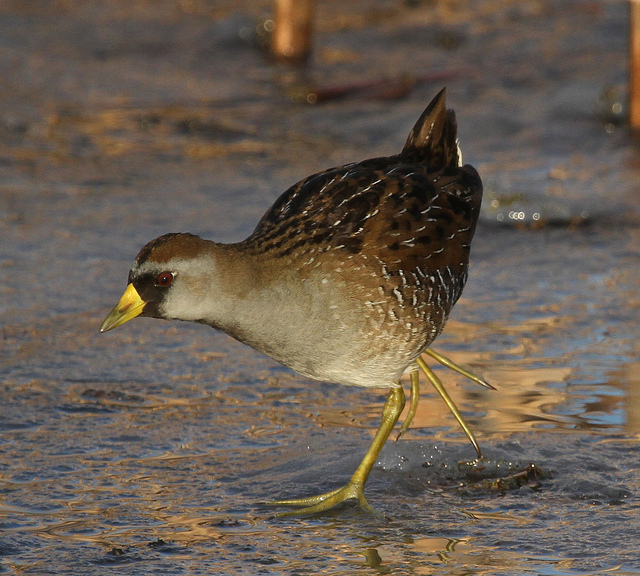
\includegraphics[width=0.4\textwidth]{figures/bird_flickr_webirdtoo}
\end{center}

\end{frame}
%%%%%%%%%%%%%%%%%%%
\begin{frame}
\frametitle{eBird}

\begin{itemize}
\item Builds on a long tradition in ornithology
\pause
\item Takes advantage of ``work'' that is already happening anyway
\pause
\item Huge amounts of data over wide geographic scale: 250,000 participants who have submitted more than 260 million bird sightings
\end{itemize}

\end{frame}
%%%%%%%%%%%%%%%%%%%
\begin{frame}
\frametitle{eBird}

\begin{center}

\includegraphics[width=0.8\textwidth]{figures/hurlbert_spatiotemporal_2012_title}
\end{center}

\vfill
\url{https://doi.org/10.1371/journal.pone.0031662}
\end{frame}
%%%%%%%%%%%%%%%%%%
\begin{frame}
\frametitle{eBird}

But, data is complex
\begin{itemize}
\item Despite input filters that remove clearly incorrect data, the data quality is unclear
\pause
\item Location of observed birds is based on location of birders
\pause
\item Heterogeneity in observer skill and protocol
\end{itemize}

\vfill
\pause
eBird data has been used in more than 200 scientific papers: \url{https://ebird.org/science/publications}

\end{frame}
%%%%%%%%%%%%%%%%%%%
\begin{frame}
\frametitle{PhotoCity}

\begin{center}
\includegraphics[width=0.6\textwidth]{figures/photocity_logo}
\end{center}

\small{
Tuite et al. (2011) ``PhotoCity: Training Experts at Large-scale Image Acquisition Through a Competitive Game'' \textit{CHI}.
}
\end{frame}
%%%%%%%%%%%%%%%%%%%%
\begin{frame}

\begin{center}
\includegraphics[width=0.6\textwidth]{figures/rome_in_a_day}
\end{center}
Rome in a Day (Agarwal et al., 2009)

\end{frame}
%%%%%%%%%%%%%%%%%
\begin{frame}
\frametitle{PhotoCity}

\begin{center}
\includegraphics[width=0.6\textwidth]{figures/tuite_photocity_2011_fig2}
\end{center}

Two campuses: University of Washington and Cornell University

\end{frame}
%%%%%%%%%%%%%%%%%
\begin{frame}
\frametitle{PhotoCity}

Over 2 months, 100,000 photos submitted by 45 players
\vfill
\begin{center}
\includegraphics[width=0.9\textwidth]{figures/tuite_photocity_2011_fig8}
\end{center}

\end{frame}
%%%%%%%%%%%%%%%%%
\begin{frame}
\frametitle{PhotoCity}

Beautiful design solves lots of problems
\begin{itemize}
\item data collection is standardized because of cameras
\pause
\item verification is automatic by comparison with nearby images
\pause
\item game points are assigned based on the value of data, trains people to collect more valuable data
\end{itemize}

\end{frame}
%%%%%%%%%%%%%%%%%%%
\begin{frame}
\frametitle{PhotoCity: Player strategies}

\begin{itemize}
\item ``[I tried to] approximate the time of day and the lighting that some pictures were taken; this would help prevent rejection by the game. With that said, cloudy days were the best by far when dealing with corners because less contrast helped the game figure out the geometry from my pictures''
\pause
\item ``When it was sunny, I utilized my camera's anti-shake features to allow myself to take photos while walking around a particular zone. This allowed me to take crisp photos while not having to stop my stride. Also bonus: less people stared at me!''
\pause
\item ``Taking many pictures of one building with 5 megapixel camera, then coming home to submit, sometimes up to 5 gigs on a weekend shoot, was primary photo capture strategy. Organizing photos on external hard drive folders by campus region, building, then face of building provided good hierarchy to structure uploads.''
\end{itemize}

\end{frame}
%%%%%%%%%%%%%%%%%
\begin{frame}
\frametitle{Malawi Journal Project}

Project:
\begin{itemize}
\item part of  Malawi Diffusion and Ideational Change Project
\item 22 citizen ``journalists'' write down all the conversations they hear about AIDS
\item 15 year timespan resulting in about 12,000 pages of text
\end{itemize}
\pause
\vfill
Result:
\begin{itemize}
\item ``journalists'' access very different knowledge than Western researchers and formal surveys
\end{itemize}

\end{frame}
%%%%%%%%%%%%%%%%%
\begin{frame}

Claims:
\begin{itemize}
\item Distributed data collection is possible for real research (eBird)
\pause
\item Sampling and data quality concerns are not insurmountable (PhotoCity)
\pause
\item Distributed data collection can produce different---not just cheaper---data (Malawi Journal Project)
\end{itemize}
 
\end{frame}
%%%%%%%%%%%%%%%%%%%%%%%%%%
\begin{frame}

What to read next:
\begin{itemize}
\item Sullivan, Wood, Iliff, Bonney, Fink, and Kelling. 2009. ``\href{https://doi.org/10.1016/j.biocon.2009.05.006}{eBird: a citizen-based bird observation network in the biological sciences}. \textit{Biological Conservation}.
\item Kaler, Watkins, and Angotti, 2015. ``\href{https://doi.org/10.2989/16085906.2015.1084342}{Making meaning in the time of AIDS: longitudinal narratives from the Malawi Journals Project}'', \textit{African Journal of AIDS Research}.
\item \textit{Bit by Bit}, \href{https://www.bitbybitbook.com/en/1st-ed/creating-mass-collaboration/design/}{Section 5.5 Designing your own}
\end{itemize}

\end{frame}
%%%%%%%%%%%%%%%%%%%%%%%%%%
\frame{\titlepage}
%%%%%%%%%%%%%%%%%%%%%%%%%%
\end{document}
